\documentclass[a4paper,11pt,twoside]{cbk} %%% Do not alter this line
 \usepackage[a4paper,portrait,inner=1.25in,outer=0.75in,top=1.125in,bottom=1.125in]{geometry}
\usepackage[colorlinks=true]{hyperref}
\usepackage[usenames,dvipsnames]{xcolor}

\usepackage{graphicx} \usepackage{setspace} \usepackage{lastpage} \usepackage{ifthen}
\usepackage{calc} \usepackage{amssymb} \usepackage{amsmath} \usepackage{amsthm} \usepackage{bm}

% uop and cms
\newcommand{\cms}{\href{http://cms.unipune.ac.in/}{Centre for Modeling and Simulation}}
\newcommand{\uop}{\href{http://www.unipune.ac.in/}{Savitribai Phule Pune University}}
\newcommand{\uopformer}{formerly \href{http://www.unipune.ac.in/}{University of Pune}}

% iitb and aero

\newcommand{\aero}{\href{http://www.aero.iitb.ac.in/home/}{Department of Aerospace Engineering}}
\newcommand{\iitb}{\href{http://www.iitb.ac.in/}{IIT Bombay}}


% logo header
\newcommand{\cmshdr}
 {
  \noindent
  \begin{minipage}{0.26\textwidth}
   \href{http://cms.unipune.ac.in/}{
\includegraphics[width=\textwidth]{cms-logo-bw}}

   \vspace*{0.5em}
  \end{minipage}
  \hfill
  \begin{minipage}{0.7\textwidth}
   \begin{flushright}
    \textsf{{\huge \cms}}

    \vspace{0.25em}
    \textsf{{\huge \uop}}

    % \vspace{0.5em}
    % \textsf{{\Large \uopformer}}

   \end{flushright}
  \end{minipage}
 }

% report front page
\newcommand{\FrontPage}
 {
  \newpage
  \thispagestyle{empty}

  \cmshdr

  \vspace{3em}
  \begin{flushright}
   {\huge \textsf{{Master of Technology (M.Tech.)}}}

   \vspace{0.5em}
   {\huge \textsf{{Programme in Modeling and Simulation}}}

   \vfill
   {\Huge \textsf{Project Report}}

   \vspace{5em}
   {\Huge \textsf{\textbf{\Title}}}

   \vspace{5em}
   {\Huge \textsf{\Author}}

   \vspace{1em}
   {\huge \textsf{\AuthorID}}

   \vfill
   {\huge \textsf{Academic Year \AY}}
  \end{flushright}

  \cleardoublepage
  % \newpage
  % ~ \vfill ~
 }

% report certificate
\newcommand{\Certificate}
 {
  \newpage
  \thispagestyle{empty}

  \cmshdr

  \setstretch{1.25}

  {\large
   \vspace{7em} \noindent
   {\Huge \textsf{\textbf{Certificate}}}

   \vspace{3em} \noindent
   This is certify that this report, titled

   \vspace{0.5em} \noindent
   \textsf{\textbf{\Title}},

   \vspace{0.5em} \noindent
   authored by

   \vspace{0.5em} \noindent
   \textsf{\textbf{\Author} (\AuthorID)},

   \vspace{0.5em} \noindent
   describes the project work carried out by the author under our supervision
   during the period from \textsf{{\DateFrom}} to \textsf{{\DateTo}}.
   This work represents the project component of the
   Master of Technology (M.Tech.) Programme in Modeling and Simulation
   at the Center for Modeling and Simulation, Savitribai Phule Pune University.

   \vspace{9em} \noindent
   {\sf
    \begin{minipage}{0.75\textwidth}
     \AdvisorA
    \end{minipage}
    \hfill
    \begin{minipage}{0.48\textwidth}
     \begin{flushright}
     \AdvisorB
     \end{flushright}
    \end{minipage}

    \vspace{8em} \noindent
    \begin{minipage}{0.48\textwidth}
     \AdvisorC
    \end{minipage}
    \hfill
    \begin{minipage}{0.48\textwidth}
     \begin{flushright}
      \Director
     \end{flushright}
    \end{minipage}
   }
  }

  \setstretch{1}

  \cleardoublepage
  % \newpage
  % ~ \vfill ~
 }

% author declaration
\newcommand{\Declaration}
 {
  \newpage
  \thispagestyle{empty}

  \cmshdr

  \setstretch{1.25}

  {\large
   \vspace{7em} \noindent
   {\Huge \textsf{\textbf{Author's Declaration}}}

   \vspace{3em} \noindent
   This document, titled

   \vspace{0.5em} \noindent
   \textsf{\textbf{\Title}},

   \vspace{0.5em} \noindent
   authored by me, is an authentic report of the project work carried out by me as part of the
   Master of Technology (M.Tech.) Programme in Modeling and Simulation
   at the Center for Modeling and Simulation, Savitribai Phule Pune University.
   In writing this report, I have taken reasonable and adequate care to ensure that
   material borrowed from sources such as books, research papers, internet, etc.,
   is acknowledged as per accepted academic norms and practices in this regard.
   I have read and understood the University's policy on plagiarism
   ({\small {\url{http://unipune.ac.in/administration_files/pdf/Plagiarism_Policy_University_14-5-12.pdf}}}).

   \vspace{8em} \noindent
   ~ \hfill \textsf{\textbf{\Author}}

   ~ \hfill \textsf{\AuthorID}

  }

  \setstretch{1}

  \cleardoublepage
  % \newpage
  % ~ \vfill ~
 }

\pagestyle{headings}
\raggedbottom
                              %%% Do not alter this line

 %%% <<<< mandatory information about this report ....
 %%%
  % report title
  \newcommand{\Title}{Validation of Rigid Body Collision Models in the PySPH Framework}

  % author
  \newcommand{\Author}{Anirudh Jonnalagadda}

  % author's ID at CMS
  \newcommand{\AuthorID}{CMS1403}

  % academic year of submission
  \newcommand{\AY}{2015-16}

  % project period
  \newcommand{\DateFrom}{January 2016} % from
  \newcommand{\DateTo}{June 2016}      % to

  % advisor 1, name and affiliation
  \newcommand{\AdvisorA} % set this to {} if not applicable
   {
    \textbf{Prabhu Ramachandran}, Professor

    Department of Aerospace Engineering

    IIT Bombay
 
    Mumbai 400 076 India

   }

  % advisor 2, name and affiliation
  \newcommand{\AdvisorB}{} % set this to {} if not applicable

  % advisor from CMS
  \newcommand{\AdvisorC}
   {
    \textbf{Sukratu Barve}, Assistant Professor

    \cms

    \uop

    Pune 411007 India

   }

  % CMS director
  \newcommand{\Director}
   {
    \textbf{Anjali Kshirsagar}, Director

    \cms

    \uop

    Pune 411007 India

   }
 %%%
 %%% .... mandatory information about this report >>>>

 % author preferences, macros, colors, etc.
 \usepackage{wrapfig}
 % \hypersetup{colorlinks,citecolor=black,filecolor=black,linkcolor=black,urlcolor=black}
 \definecolor{turquoise}{HTML}{06959b}
 \definecolor{manpurple}{rgb}{0.419607843,0.1725490196,0.56862745098}
 \usepackage{amsmath}
 \usepackage{hyperref} 
 \usepackage{minted}
 \usepackage{subcaption}
 \usepackage{array}
 \usepackage{listings}
 \usepackage{tikz}
 \usetikzlibrary{shapes,arrows}

 \newcolumntype{L}{>{\centering\arraybackslash}m{10cm}}

 \lstset
 {
    basicstyle=\small\ttfamily,
    commentstyle=\color{Green},
    keywordstyle=\color{Cerulean},
    frame=L,
    language=python,
    morekeywords={True, False},
    numbers=left,
    numbersep=10pt,
    numberstyle=\footnotesize\color{Gray},
    showstringspaces=false,
    stringstyle=\color{Mulberry},
    tabsize=3,
 }

\begin{document}

 %%% <<<< mandatory initial pages ....
  \FrontPage
  \Certificate
  \Declaration
 %%% .... mandatory initial pages >>>>

 \chapter*{Abstract}

Problems incorporating both solid-fluid and solid-solid interations are prevalent in a large number of engineering disciplines. Traditional approches using Eulerian approaches suffer on account of having to keep track of, and accurately capture the complicated solid-fluid interfaces. A fairly established numerical scheme to model solid-solid interactions is that of the Discrete Element Method (DEM). Further, recent attempts to use meshfree particle methods such as Smoothed Particle Hydrodynamics (SPH) for fluid flow problems have shown encouraging results.

Both the DEM and SPH, being particle methods, seem to be good candidates for integration, whence a robust and fully Lagrangian formulation can be realised. PySPH, an open source Python based framework to perform Smoothed Particle Hydrodynamics simulations, being notoriously user and developer friendly is the mouthpiece of choice in which such an integration is attempted.

The present work first elucidates the structure of the PySPH framework, describes a simple DEM based Rigid Body Collision Model, followed by its Proof of Concept implementation in PySPH . Thereafter, a numerical validation study performed to ascertain the physical consistency of the model is detailed; it is followed by the description of an optimized Collsion model based on recent research endeavours and the development of an algorithm to implement in PySPH. Finally the implementation in the PySPH framework is discussed.

 \addcontentsline{toc}{chapter}{Abstract}

 \chapter*{Acknowledgments}

My time at the Centre was underscored by innumerable priceless encounters with a number of inspirational individuals. I am glad that I have a opportunity to express my gratitude for their invaluable contributions.

First and foremost, a big thank you to Dr. Prabhu Ramachandran of the Department of Aerospace Engineering at IIT Bombay. Not only has he been instrumental in introducing me to a unique and challenging topic to pursue as part of my Masters Project, but he has also always available to mentor, guide and advise me; this, despite the obvious constraints of distance, personal and professional commitments and a visibly jam-packed schedule. My interactions with Prabhu Sir have always helped me to see things in fresh light; it was really a pleasure to have had the opportunity to work and interact with him.

Another large, ubiquitous calming presence at CMS was that of Dr. Sukratu Barve. The knowledge that I could always bank on Barve Sir for academic and/or other kinds of guidance was very reassuring. As my Guide at CMS, we had countless fruitful discussions, many of which continued well past normal office hours. My heartfelt gratitude for all his suggestions, comments and insights.

Further notable mentions are that of Dr. Mihir Arjunwadkar and Dr. Jayaraman Valadi. Mihir Sir has been kind and encouraging from the very beginning. Conversations with him would always be candid and at the same time extremely enlightening and motivating. Jayaraman Sir, with his vast experience, brought to the table a wealth of knowledge. Any interaction with him left me knowing a little more than I had before. Thanks to them, monotonously mundane days became enjoyable.

Finally, my friends (you know who you are), my sisters, Drs. Mallika and Manjari Jonnalagadda, my brothers-in-law, Saju Jospeh and Shantanu Ozarkar and my parents, Kedarnath and Rama Jonnalagadda have been a pillar of support through thick and thin. It is only with their love and support that I could be in a position to successfully complete this endeavour. Also, an eternal source of joy in those inevitable times of stress came in the shape and form of my nephews Siddhartha and Anay; they too have played a big role in their own little way.

\vfill
\noindent
{\large{Copyright \copyright \space 2016 | Anirudh Jonnalagadda\\All rights reserved}}

 \addcontentsline{toc}{chapter}{Acknowledgments}

 \tableofcontents

 \chapter{Introduction}

The use of mathematical models for modelling the behaviour of physical systems has prevailed for as long as one can remember. For typical fluid flow problems, the equations obtained using the Continuum Approximation are most widely used; the yardstick for rigid bodies are the Newton's Laws of Motion. In the case of Isotropic Newtonian fluids, the flow equations boil down to the popular form as given by Navier and Stokes. More often than not, these equations and the associated boundary conditions describing the physical systems of interest, are intractable and do not produce any closed form mathematical expression; thus, one resorts to approximating the variables associated with the system by means of Numerical Methods. Further, the physical systems this work aims to tackle involve solid-solid as well as solid-fluid interactions along with fluid flow; such problems are broadly classified as ``Fluid Structure Interaction (FSI)'' problems. FSI situations are extensively encountered in a number of engineering scenarios spanning a large number of domains and, hence, the ability to accurately capture all three types of interactions is paramount.

A plethora of Numerical Methods are available to model fluid flow; most widely used are those of the Finite Difference Method (FDM), the Finite Volume Method (FVM) and Finite Element Method (FEM). However, these popular methods build on an Eulerian framework and require the problem domain to be discretized explicitly into a grid. In contrast, Particle Methods (also called as Grid/Mesh Free methods) work with a Lagrangian framework and do not demand for domain discretization via a grid. The Smooth Particle Hydrodynamics (SPH) method is one such particle method.

To resolve the forces acting on interacting solid bodies, the Discrete Element Method (DEM) employing various contact models (Soft Contact Models and Hard Contact Models) have been successfully used. Hard Contact Models take into consideration the Coefficient of Restitution of the interacting bodies to estimate the collision force. However for large number of situations, experimental computations of the coefficient of restitution is often tedious, and at times practically untenable. On the other hand, Soft Contact Models allow the interacting bodies to ``merge'' into one another, and using the amount of overlap as the displacement to a spring and damper system, estimate the Collision Forces.

After obtaining the Collision forces, Newton's Laws of Motion are solved to obtain the positions, (linear as well as angular) velocities and accelerations of system of solids thus ending one iteration of the solid-solid interaction. Thereafter, by means of a coupling mechanism, these details are communicated to the fluid, wherein appropriate source terms are incorporated to accommodate the effect of collision. Subsequently, SPH takes over to obtain flow properties. This completes one iteration of the integrated model. The coupling mechanism and the flow field solution obtained using SPH is beyond the scope of this work; the major concentration is on implementation of DEM based Collision models in PySPH. However, for the sake of understanding both the design philosophies of the PySPH tool and the SPH numerical method itself, the SPH method is discussed in a (sufficiently) brief introductory capacity.

The remainder of the report is laid out as follows: Chapters 2 and 3 discuss the details of the SPH and DEM numerical methods and the PySPH framework respectively. Chapter 4 describes a DEM method inspired Proof of Concept (PoC) collision model, its implementation in PySPH and a study performed to validate the model; the chapter is closed off with qualitative results to demonstrate shortcomings of the PoC model. Thereafter, in Chapter 5, an improved model is presented along with an algorithm for its implementation in PySPH. The report concludes with avenues that can be explored to carry out robust simulations for FSI problems with PySPH. % introduction
 \chapter{Numerical Methods}
%

This chapter discusses the Smoothed Particle Hydrodynamics (SPH) and the Discrete Element Method (DEM) numerical methods.

\section{Smoothed Particle Hydrodynamics}

The Smoothed Particle Hydrodynamics (SPH) numerical method was developed in the late 1970s \cite{gingold_monaghan} for tackling problems in Astrophysics which involved arbitrarily moving, three dimensional fluid masses in the absence of boundaries; the equations represented below are discussed in this framework. Since it's inception however, the SPH method has come a long way and has been used in numerous fields such as magneto-hydrodynamics, multi-phase flows, quasi-incompressible flows, gravity currents, flow through porous media, heat conduction, shock simulations, heat transfer and mass flow, explosion phenomenon, high/hyper velocity impact problems etc.

\begin{figure}[htb!]
\centering
\setlength\fboxsep{0pt}
      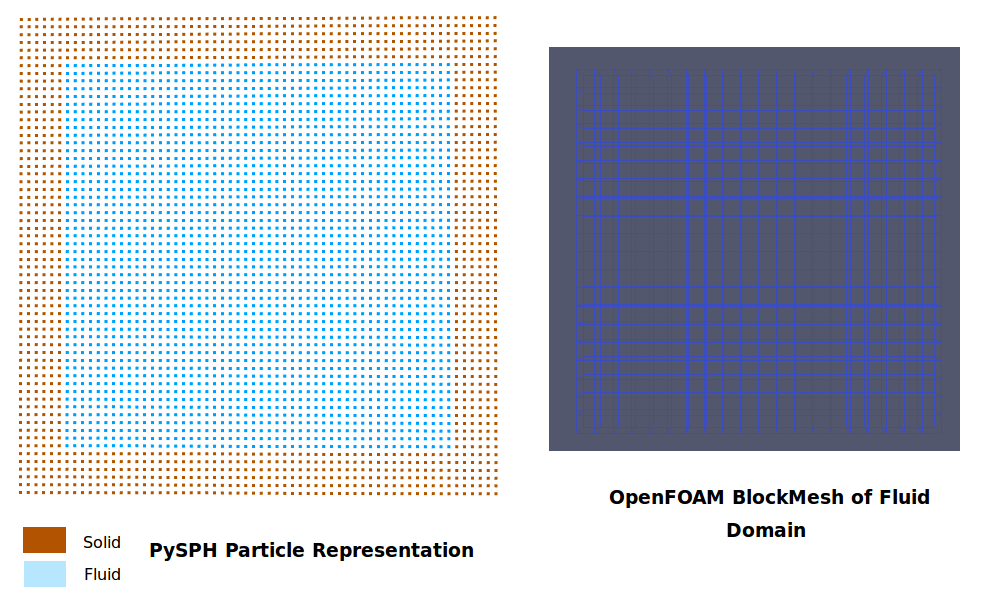
\includegraphics[width=5in, height=2.5in]{figures/particle_rep.png}
\caption{{\small{Domain Discretization in the SPH and FVM numerical Methods}}}
\label{fig:particle_representation}
\end{figure}

The SPH method takes into account the motion of a set of points whose velocity and thermal energy is known at all times. These points are also assigned a mass, and hence, are called as ``Particles''\cite{monaghan_intro}. Thus Domain discretization is achieved by means of a ``Particle Representation'' which describes the fluid domain. Such a representation allows for a completely arbitrary initial distribution of particles, with no explicit requirement of inter-particle connectivity, thereby qualifying SPH to be a Mesh-Free numerical method. Figure ~\ref{fig:particle_representation} shows the domain discretization for a simple incompressible flow problem (the lid-driven cavity) for solving equations with the SPH method and the Finite Volume Method (FVM). The software tools used for generating the representations are PySPH \cite{prabhu_puri} and OpenFOAM respectively.

Every particle has all the field variables of a Continuum Point Particle associated with it\footnote{``Particles'' are an outcome of the application of SPH on the matter continuum;``Point Particles'' are the basic building blocks of the Continuum approximation.}. The SPH method represents the governing differential equations as a set of difference equations with the dependant and independent variables of the differential equations being related to those ~ of ~ the ~ difference ~ equation ~ by ~ means ~ of ~ a ~``Particle ~ Approximation'' ~ \cite{sph:volieu}\\\cite{liu_liu} detailed below.

\subsection{Particle Approximation}\label{kappa}

Consider an arbitrary scalar field A(\textbf{r},\textit{t}) associated with a particle having position vector \textbf{r} at time \textit{t}. This field can be written as a spatial convolution with the Dirac Distribution $\delta$ as, 

\begin{eqnarray} \label{eq:dirac}
 A(\textbf{r},\textit{t}) &=& (A\ast \delta)(\textbf{r},t) \nonumber \\
                          &=& \int_{\varOmega} A(\textbf{r'},t) \delta (\textbf{r - r'}) d^{3}\textbf{r'} 
\end{eqnarray}

where $\varOmega$ represents the domain of the Continuum. 

Practically, the Dirac Distribution is approached by use of Interpolation Kernels\footnote{The terms Interpolation Kernels, Mollifiers, Smoothing Kernels etc. are used interchangeably in literature.}, denoted as \textit{w$_h$}(\textbf{r - r'}). These kernels could have a compact or an infinite support and have associated with them a Smoothing Parameter ``h'' which controls the sphere of influence of each particle. For a kernel with a compact support, if the point particle under consideration were imagined to be at the center of an n-dimensional hypersphere (n$=$3 in this particular case) of radius, \textit{r}$=\kappa$h ($\kappa$ being a multiplying constant), then all those point particles which lie within this hypersphere would contribute to the properties of the point particle at the center; for a kernel with an infinite support, the effect of point particles at larger distances from the center of the hypersphere would diminish. Thus, the continuous domain of integration $\varOmega$ is reduced to that of the the hypersphere, $\varOmega_r$. (Properties of Kernels are discussed in \ref{ssec:kernels}). 

\begin{figure}[htb!]
\centering
\setlength\fboxsep{0pt}
      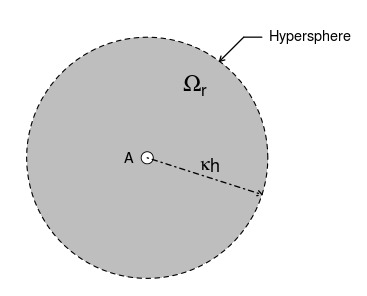
\includegraphics[scale=0.6]{figures/SpInfContinuous_R.png}
\caption{{\small{Sphere of Influence of a Point Particle A centred at the Origin of a 2D Hypersphere}}}
\label{fig:sphere_influence}
\end{figure}
\newpage
Equation \eqref{eq:dirac} can be rewritten, by making the ``Kernel Approximation'',  as,

\begin{eqnarray} \label{eq:continuous-approximation}
 A(\textbf{r},t) \approx [A]_{c}(\textbf{r},t)= \int_{\varOmega_r} A(\textbf{r'},t) \textit{w$_h$(\textbf{r - r'})} d^{3}\textbf{r'}
\end{eqnarray}

Equation \eqref{eq:continuous-approximation} is called the Kernel/Continuous Approximation of the field A(\textbf{r},\textit{t}) which is introduced due to the use of the Kernel function \textit{w$_h$}(\textbf{r - r'}).

Thereafter, a discrete interpolation is obtained by expressing Equation \ref{eq:continuous-approximation} as a Riemann sum over all the particles falling within the hypersphere, i.e.

\begin{eqnarray} \label{eq:particle-approximation}
     [A]_{c}(\textbf{r},t) &=& \int_{\varOmega} A(\textbf{r'},t) \textit{w$_h$(\textbf{r - r'})} d^{3}\textbf{r'} \nonumber \\
     &\approx & \sum_{b}A(\textbf{$\bf{r}_b$},t)~\textit{w$_h$}(\textbf{$|\bf{r}-\bf{r}_b |$}) ~ \textit{V$_b$} = [A]_{d} \nonumber \\
     \therefore [A]_{d} &=& \left( \sum_{b}A(\textbf{$\bf{r}_b$},t)~\textit{w$_h$}(\textbf{$|\bf{r}_{ab} |$}) ~ \textit{V$_b$}\right) ,
     \forall a \in  \varOmega_r , \textbf{r}_{ab} = \textbf{r}_{a} - \textbf{r}_{b}
\end{eqnarray}

The job of keeping track of all the particles ``b'' which influence any particle ``a'' is designated to the a Nearest Neighbour Particle Search (NNPS) Algorithm. Although the NNPS is the main work-horse of any SPH simulation, its description and implementations is beyond the scope of this work. 

To conclude, it should be noted that although the treatment given above is for an arbitrary scalar field, the same can be extended to an arbitrary vector field as well, by treating each component individually. Furthermore, the above treatment is valid only for the bulk of the fluid in the absence of any boundaries; treatment of boundaries within SPH is addressed separately and is not discussed in this work.

\subsection{Kernel Functions} \label{ssec:kernels}

This section describes the main properties a kernel function should possess in order to be able to produce the first order accurate description given in Equation \eqref{eq:continuous-approximation}.

\subsubsection{Kernel Properties}
 The two conditions on imposed a kernel function are:
 \begin{eqnarray} \label{eq:kernel-props1} 
  \int_{\varOmega_0} \textit{w$_h(\widetilde{r}) ~d^{3}\widetilde{r}$} = 1
 \end{eqnarray}
 and
 \begin{eqnarray}\label{eq:kernel-props2}
  \int_{\varOmega_0} \textit{w$_h(\widetilde{r})~ \widetilde{r}~ d^{3}\widetilde{r}$} = 0 
 \end{eqnarray} 
 where ${\varOmega_0}$ is ${\varOmega_r}$ translared to the origin \textbf{0}.
 

 Equation \eqref{eq:kernel-props1} stipulates that the zeroth order moment (i.e. the Mean or the Expectation) of the Kernel be 1, like that of the Dirac $\delta$; \eqref{eq:kernel-props2} stipulates that the first order moment (i.e. the Variance) be zero. 
 
 There are various ways in which, mathematically, one could construct functions which satisfy the above two requirements. However, in general, the simplest way to satisfy \eqref{eq:kernel-props2} is by using a Symmetric function (which could be normalized to ensure \eqref{eq:kernel-props1} is satified as well). \newpage This gives us the following relation for the Kernel function:
 
 \begin{eqnarray}\label{eq:kernel-symmetry}
  \textit{w$_h(\widetilde{r}$)} = \textit{w$_h(-\widetilde{r}$)}
 \end{eqnarray}

\section{Discrete Element Method} \label{sec:DEM}

The Discrete Element Method \cite{mishra} is a numerical method that allows finite rotations and displacements of discrete bodies which interact with their nearest neighbours by means of local Contact Laws where the loss of contact and the formation of new contacts occur as the simulation progresses. To track the position of the solid rigid bodies, the interacting bodies (also called as particles) are modelled as a dynamic process in which contacts are broken and formed. In order to estimate the reaction force due to interaction or collision between particles ``Hard'' or ``Soft'' Contact models are employed. Hard Contact models rely on the phenomenon of Restitution and require information of the Coefficient of Restitution between the interacting particles to be supplied as a model parameter. Since obtaining information about the Coefficient of Restitution experimentally is quite an arduous task, Hard Contact models are not widely used. Soft Contact Models, on the other hand, allow the particles to overlap during contact. The amount and rate of overlap gives rise to an incremental force which is tracked in each calculation cycle. Thereafter, numerical integration of Newton's Second Law of Motion gives the linear and angular velocities of the system; a second integration gives the linear and angular displacements.

The DEM method requires the net unbalanced forces to be calculated for all particles on account of interaction with all other particles within the system. In the case of an interaction, the resulting force will be non-zero, otherwise the resulting force will be zero for that particular pair of interacting particles. However, for a system comprising of \textbf{N} particles, this would result into keeping track of $\dfrac{{\bf{N}} \times {\bf{(N-1)}}}{2}$ interactions. In order to improve the efficiency of the computation, the entire working area is divided into squares (or cubes depending on whether a 2/3 dimensional implementation is being considered). Such a procedure is called as ``Boxing'' in the DEM literature. Generally, the dimension of the box is the diameter\footnote{In general, DEM particles are taken to be spherical; however, there are many studies made for particles of different shapes.} of the largest particle in the system. A particle is regarded as a member in all those boxes where the corners of its circumscribing square have an entry.  A list of all the particles in a box (i.e. a Box List) is generated and only those elements which have entries in a box are considered for potential contact. Thereafter, soft contact models are (generally) employed, and the incremental force is computed. % Numerical Methods
 \chapter{PySPH: Design Philosophy}

PySPH ~\cite{prabhu_puri} ~ is ~ an ~ open-source, ~ objected ~ oriented ~ Python\\ \cite{python} based framework for SPH simulations with the performance critical portions implemented in Cython \cite{cython}. The PySPH tool is flexible, user-friendly and allows for quick prototyping and extension to new problems. In this chapter, a broad outline of the PySPH tool is laid out\footnote[4]{further details of specifics related to new implementations will be discussed as and when encountered}.

\section{Abstractions for Numerical Implementation} \label{sec:pysph_abstractions}

In order to motivate and explain the abstractions made for the numerical implementation, we consider a general SPH discretization (Equations \eqref{eq:Disc_SPH}) for the continuum equations for Mass, Momentum and Energy balance (Equations \eqref{eq:balance_laws}):

\begin{eqnarray} \label{eq:balance_laws}
\frac{D\rho}{Dt} &=& -\frac{1}{\rho} \nabla \cdot \vec{v} \nonumber \\
\frac{D{\vec{v}}}{Dt}&=&\vec{k} + \frac{1}{\rho} \frac{\partial \tau^{lm}}{\partial x_m} \hat{l} \\
\frac{D{\it{e}}}{Dt}&=& -\frac{1}{\rho}\nabla \cdot \vec{q} + \frac{1}{\rho}\frac{\partial {\it{v}^{l}} }{\partial x_m}\tau^{lm} \nonumber
\end{eqnarray}

{\raggedright{where,}}\\
$\frac{D}{Dt}(\varphi) = $ Material Derivative of the field variable $\varphi = \left(\frac{\partial}{\partial t} + \vec{v}\cdot\nabla\right)(\varphi)$ \\
$\rho = $ Mass per unit volume in the limit that volume goes to zero at any point in the continuum\\
$\vec{v} = $ Velocity vector associated with a point particle\\
$\vec{k} = $ Body Force per unit mass\\
$\tau^{lm} = $ Components of the stress tensor field\\
$e = $ Internal Energy per unit mass\\
$\vec{q} = $ Heat Flux Vector (heat energy transferred per unit time per unit area along the direction of heat flow) 

\newpage

\begin{eqnarray}\label{eq:Disc_SPH}
 \frac{D\rho_{a}}{Dt} &=& \sum_{b \in \Omega_{r}} m_{b}{\mathcal{D}}_{ab}(\vec{v})\cdot {\nabla}_{i} W_{ab}(h) \nonumber \\
 \frac{Dv^{i}_{a}}{Dt} &=& \sum_{b \in \Omega_{r}} m_{b}{\mathcal{F}}_{ab}(\rho ,P,\vec{v})\frac{\partial}{{\partial x}^{i}}W_{ab}(h)\\
 \frac{De_{a}}{Dt} &=& \sum_{b \in \Omega_{r}} m_{b}{\mathcal{E}}_{ab}(\rho ,P,\vec{v}) \cdot W_{ab}(h) \nonumber
\end{eqnarray}

{\raggedright{where,}}\\
${\rho}_a = $ Density of the particle ``a'' \\
$\Omega_{r} = $ Hypersphere of Influence of radius $\kappa$h\\
$m_b = $ mass of the particle ``b''\\ 
$v^{i}_{a} = i^{th}$ component of velocity of the particle ``a'' \\
$W_{ab} = $ Smoothing Kernel\\
$e_a = $ Internal Energy per unit mass of the particle ``a''\\

Referring to Figure \ref{fig:nearest_neighbors}, we see how the properties of a particle ``a'' evolves via its interaction with nearest neighbours represented by particles ``b'' in the hypersphere $\Omega_{r}$; the descriptions of the terms $\kappa$ and ``h''  are given in section \ref{kappa}

\begin{figure}[htb!]
\centering
\setlength\fboxsep{0pt}
      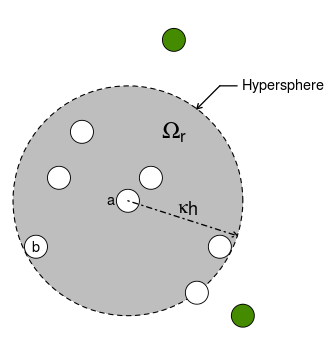
\includegraphics[scale=0.6]{figures/SpInfDiscrete_R.png} 
\caption{{\small{Neighbors List for a Particle ``a''}}}
\label{fig:nearest_neighbors}
\end{figure}

The terms $\mathcal{D}, \mathcal{F}$ and $\mathcal{E}$ are representations of the ``fluxes'' of mass, momentum and energy which contribute to the properties of particle ``a''. Based on the (non-exhaustive) discretizations given in Equations \eqref{eq:Disc_SPH}, PySPH incorporates the following abstractions:

\begin{itemize}
\item \textbf{\textit{Particle Container: }}It is the data structure which represents the arbitrary collections of particles inherent to the SPH method. The material species is represented as a collection of arrays (i.e. contiguous blocks of memory) describing the required properties. The default particle container comes with representations for the position, velocity, acceleration, pressure, mass, smoothing length and density along with a unique global index(gid), processor id(pid) and a tag\footnote[5]{\url{http://pysph.readthedocs.io/en/latest/reference/particle_array.html}}. Additional properties, if required, can be easily added on the fly. 

\item \textbf{\textit{Nearest Neighbour Queries: }} As mentioned in Section \ref{kappa}, the keeping track of the nearest neighbours of any particle as specified by the hypersphere of influence(Figure \ref{fig:nearest_neighbors}) is computationally the most costly aspect of an SPH simulation. For performing such queries, Nearest Neighbour Particle Search (NNPS) Algorithms are used. By default PySPH implements a Linked List based NNPS; there are however a few more implementations to choose from\footnote[6]{\url{http://pysph.readthedocs.io/en/latest/reference/nnps.html}}.

\item \textbf{\textit{Interaction Physics: }}Based on the specific application area, the physics of the problem defines the nature of the general interaction terms  $\mathcal{D}, \mathcal{F}$ and $\mathcal{E}$ appearing in Equations \ref{eq:Disc_SPH}; there may also be inclusions of viscous stress and artificial viscosity terms for numerical stability of the scheme (more information of details for SPH in specific applications could be found at e.g. \cite{price}, \cite{monaghan_ARFM}, \cite{monaghan_physics},  \cite{volker_springel}). The Interaction Physics abstraction defines these general interaction terms in the context of ``solving'' Equations \ref{eq:Disc_SPH} to obtain the accelerations of the particles.

\item \textbf{\textit{Integrator: }}Post completion of the particle interactions, the solution is updated in time using an Integrator\footnote[7]{\url{http://pysph.readthedocs.io/en/latest/reference/integrator.html}} step. These integrators can include multiple-stages wherein intermediate storage of the properties is inherently available. 

\item \textbf{\textit{Miscellaneous: }}Lastly, data structures, routines and tools to construct solvers, equations, post process the results etc. are required. For post processing, the Mayavi\footnote[8]{\url{http://code.enthought.com/projects/mayavi/}} tool is utilized whereas all other requirements are addressed via routines in the source-code.
\end{itemize} 

\section{Design}\label{sec:pysph_design}

Although superficially it may look like PySPH is written in Python, it is, in reality, a blend of multiple languages. Cython is used to implement the performance critical neighbour queries and pair-wise force computations by creating C/C++ extensions. Further PySPH implements Run Time Code Generation (RTCG) i.e. any case setup using PySPH is inherently converted into C/C++ extensions using Cython. This ascribes PySPH it's computational edge. Distributed memory computations can be performed via MPI using the Python binding mpi4py \cite{mpi4py} and dynamic load balancing is achieved through the Zoltan data management library \cite{zoltan} via a custom Python wrapper. PySPH can also be seamlessly integrated to use OpenMP for speed-up on systems with multiple cores.

\begin{figure}[htb!]
\centering
\setlength\fboxsep{0pt}
      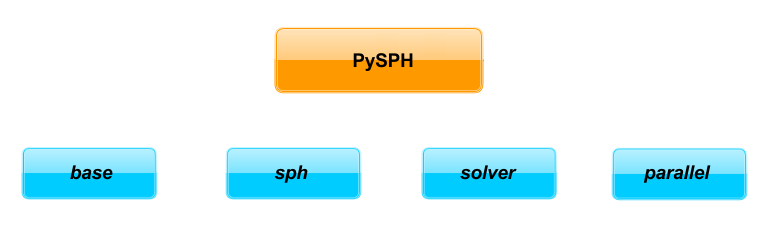
\includegraphics[scale=0.35]{figures/pysph_modules.png} 
\caption{{\small{PySPH subpackages (reproduced from \cite{prabhu_puri})}}}
\label{fig:pysph_modules}
\end{figure}

PySPH comprises of four subpackages as shown in Figure \ref{fig:pysph_modules}. The \textit{base} subpackage contains definitions for the data structures for the particle arrays and nearest neighbour queries on particle sets. The \textit{sph} subpackage contains definitions related to the ``physics'' of the problem. The user's entry point into PySPH is through the  \textit{solver} subpackage wherein provisions are made to facilitate solver construction, choice of the time-stepping scheme and setting of solver parameters. Lastly, the \textit{parallel} subpackage takes care of the domain decomposition, load balancing and computation of remote neighbours using MPI.

Figure \ref{fig:sph_algo}\footnote[9]{\url{http://pysph.readthedocs.io/en/latest/tutorial/circular_patch_simple.html}} describes the general procedure to setting up a SPH simulation using PySPH.  

\begin{figure}[htb!]
\centering
\setlength\fboxsep{0pt}
      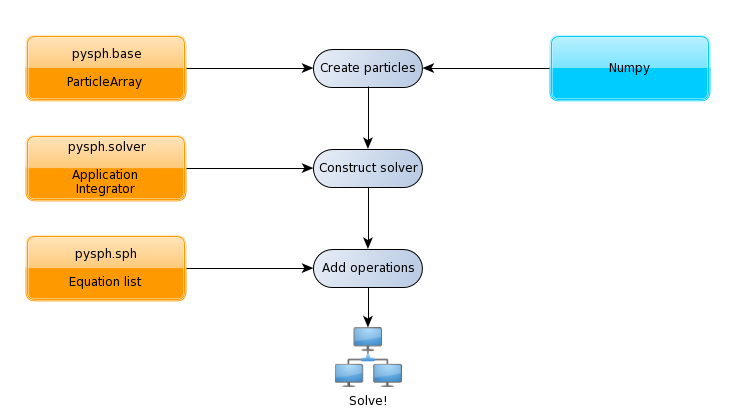
\includegraphics[scale=0.5]{figures/pysph-examples-common-steps.png} 
\caption{{\small{Common Steps (reproduced from PySPH Documentation)}}}
\label{fig:sph_algo}
\end{figure}

To begin with, using Numpy functions in conjunction with the ParticleArray convenience functions Domain Discretization, is performed. Subsequently, the solver is set up wherein details of the Kernel, time step, end time, write frequency etc. are specified along with the choice of integrator scheme to be used. Thereafter, equations which define the interaction physics are constructed and finally solved either serially or in parallel. 
 % PySPH
 \chapter{PySPH and DEM}

The Discrete Element Method, being a particle method, has attributes which allow for an implementation in the PySPH framework. These attributes, introduced in section \ref{sec:DEM}, are:

\begin{itemize}
\item Representation of the Solid Bodies as ``particles''.
\item Efficient search of particles coming into contact with one another via Boxing and Contact Searching.
\end{itemize}

In PySPH, the solid bodies can be represented as a collection of particles assigned with a ``body tag'' to demarcate the individual solid entities. Further, for neighbour search, the hypersphere of influence is analogous Boxing. Lastly, contact can then be established by using contact models and the contact forces can be computed. Thus, conceptually, a DEM implementation in PySPH should be possible.

This chapter describes a Soft Contact model and it's PySPH implementation. Thereafter, a case study performed to validate the collision model is described. Finally, the conclusions of the validation study are presented.

\section{Validation of the RigidBodyCollision Model}

This model \cite{gpu_gems}\footnote[10]{\url{http://http.developer.nvidia.com/GPUGems3/gpugems3_ch29.html}} represents the Proof of Concept establishing that DEM can be implemented in PySPH. It models the contacts as a Spring and Dashpot system as follows:

\begin{eqnarray}\label{eq:RigidBodyCollision}
Repulsive Force, f_{i,s} &=& -k~(d-|{\bf{r_{ij}}}|)~\frac{{\bf{r_{ij}}}}{|{\bf{r_{ij}}}|} \nonumber\\
Damping Force, f_{i,d} &=& \eta ~ {\bf{v_{ij}}} \\
Shear Force, f_{i,t} &=& k_{t}~{\bf{v_{ij,{\it{t}}}}} \nonumber
\end{eqnarray}

{\raggedright{where},} \\
{\it{k}} $=$ Spring Coefficient $\hspace{0.375cm}$ ; $\hspace{0.375cm}$ {\it{k$_t$}} $=$ Coefficient of Shear $\hspace{0.375cm}$ ; $\hspace{0.375cm}$ $\eta =$ Damping Coefficient\\
d $=$ diameter of elements comprising the body\\ 
${\bf{r_{ij}}} = \textbf{r}_{i} - \textbf{r}_{j}$ $\hspace{0.375cm}$ ; $\hspace{0.375cm}$ ${\bf{v_{ij}}} =\textbf{v}_{i} - \textbf{v}_{j} $ \\
Relative Tangential Velocity, ${\bf{v_{ij,{\it{t}}}}} = {\bf{v_{ij}}} - \left({\bf{v_{ij}}} \cdot \frac{{\bf{r_{ij}}}}{|{\bf{r_{ij}}}|}\right) \frac{{\bf{r_{ij}}}}{|{\bf{r_{ij}}}|} $\\

In order to validate the RigidBodyCollision Model, a comparison with experimental results published by \cite{zhang} is made. The experimental set up consisted of an acrylic resin tank with dimensions of 26 cm $\times$ 10 cm $\times$ 26 cm (L$\times$B$\times$H) with solid aluminium cylinders of diameter 1 cm, length 9.9 cm, and density 2.7 $\times$ 10$^3$ $\frac{kg}{m^3}$ stacked in horizontal layers as shown in Figure \ref{fig:exp_setup}. The system is held in equilibrium by a plate which is removed to begin the experiment. The state of the system for a 6 layer cylinder stack (Figure \ref{fig:sys_state}) is captured using a High Speed camera shooting at 200 frames per second. Also, the evolution of the average mass centers of the six cylinder collapse is plotted (Figure \ref{fig:sys_cm}) after 5 experimental trials.

\begin{figure}[htb!]
\centering
\setlength\fboxsep{0pt}
      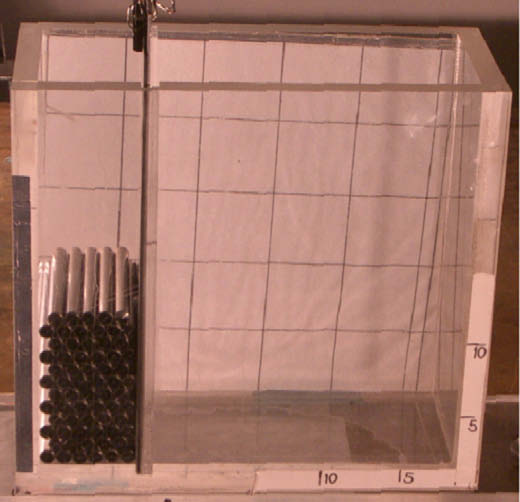
\includegraphics[scale=0.3]{figures/exp_setup.png} 
\caption{{\small{Experimental Setup (reproduced from \cite{zhang})}}}
\label{fig:exp_setup}
\end{figure}

\begin{figure}[htb!]
\centering
\setlength\fboxsep{0pt}
      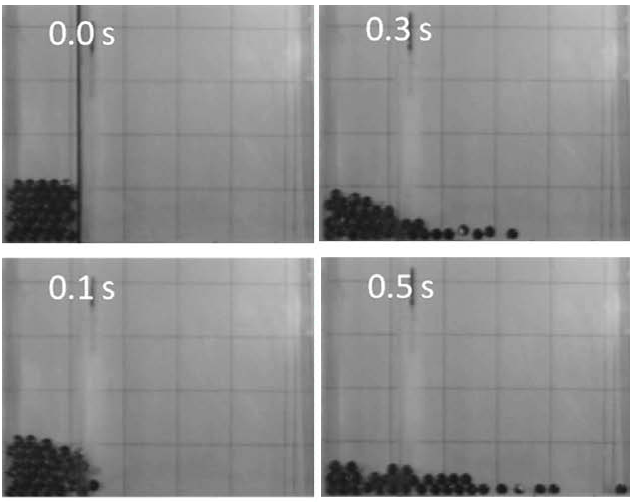
\includegraphics[scale=0.3]{figures/sysEvol.png} 
\caption{{\small{Evolution of 6 Cylinder Stack (reproduced from \cite{zhang})}}}
\label{fig:sys_state}
\end{figure}

\begin{figure}[!htb]
\centering
\setlength\fboxsep{0pt}
       \begin{tabular}{cc}
 	   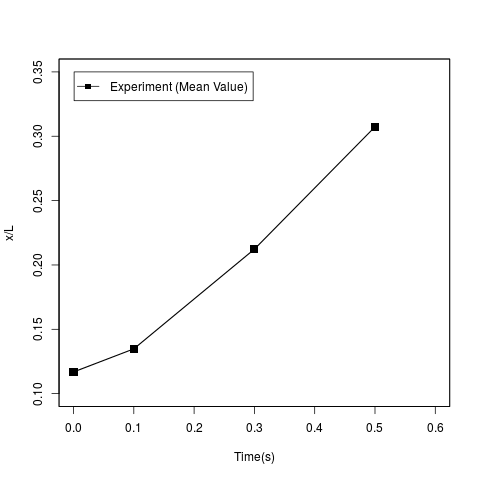
\includegraphics[scale=0.325]{figures/XexpDataR.png} &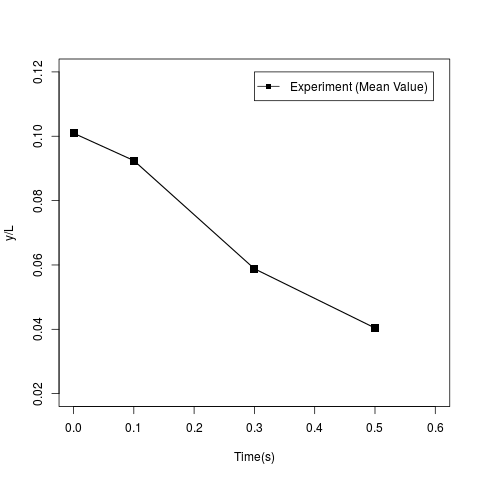
\includegraphics[scale=0.325]{figures/YexpDataR.png}
 	   \end{tabular}      
\caption{{\small{Six Cylinder System Center of Mass (x, y are the center of masses in the X and Y directions) (reproduced from \cite{zhang})}}}
\label{fig:sys_cm}
\end{figure}

The ~ 6 ~ cylinder ~ case ~ is ~ set ~ up ~ in ~ PySPH ~ via ~ the ~ ``\_create\_geometry.py'' ~ and the ``rigid\_body\_validation.py'' (\ref{app1:case}) programs respectively. The particles are created using the \lstinline!create_particles()! method in the \lstinline!class CollapsingCylinderGeometry()!, the solver is created using \lstinline!create_solver()! method and the interaction physics is defined in the \lstinline!create_equations()! method, from the \lstinline!class CollapsingCylinder()!; a body force of 981 $\frac{cm}{s^2}$ is imparted in the $-Y$ direction, collisions are modelled and Newton's Equations for Rigid Body Dynamics (Equation \ref{eq:newton}) are solved.

\begin{eqnarray}\label{eq:newton}
Rigid Body ~{\textit{\textbf{I}}} &=& \left\lbrace particles : r_{ij} = 0, ~ \forall t , i,j \in I\right\rbrace \nonumber \\
M_{I}\frac{d{\it{{\bf{V_I}}}}}{dt} &=& \sum_{k~\in~I} m_{k} \frac{d{\it{{\bf{v_k}}}}}{dt} \\
{\bf{\it{I_I}}} \frac{d{\bf{\varOmega _{I}}}}{dt} &=& \sum_{k~\in~I} m_{k}\left( {\bf{r_k - R_I}}\right) \times \frac{d{\it{{\bf{v_k}}}}}{dt} \nonumber
\end{eqnarray}

{\raggedright{where,}} \\
$M_I , {\it{\bf{V_I}}}, {\it{\bf{R_I}}} = $ Mass, Velocity and Center of Gravity of {\it{``I''}}, \\
$I_I , {{\bf{\varOmega _{I}}}} = $Inertial Tensor(Moment of Inertia), Angular Velocity of {\it{``I''}} \\
$m_k , {\it{{\bf{v_k}}}}, \bf{r_k} =$ Mass, Velocity and Position of $k^{th}$ particle\\

The case set up in PySPH is shown in Figure \ref{fig:sim_setup}. Among the various parameter combinations tried, the best results were obtained for the parameter values of $k = 8.0, d = 2.5, \eta = 0.01$ and $k_t = 0.1$. However, a qualitative inspection of the simulation shows that the model is physically inconsistent. A snapshot of the simulation at time $t = 0.032s$ is shown in Figure \ref{fig:bestresult_snapshot} where the cylinder arrays can be seen to merge into one another. A possible explanation for the failure of the model could be that there is no description of the material properties of the interacting solid bodies which would definitely play a vital role in the collision process. This observation leads us to move on to the search of a better suited model, which is further detailed in the next chapter.

\begin{figure}[htb!]
 \begin{subfigure}{.5\textwidth}
  \centering
    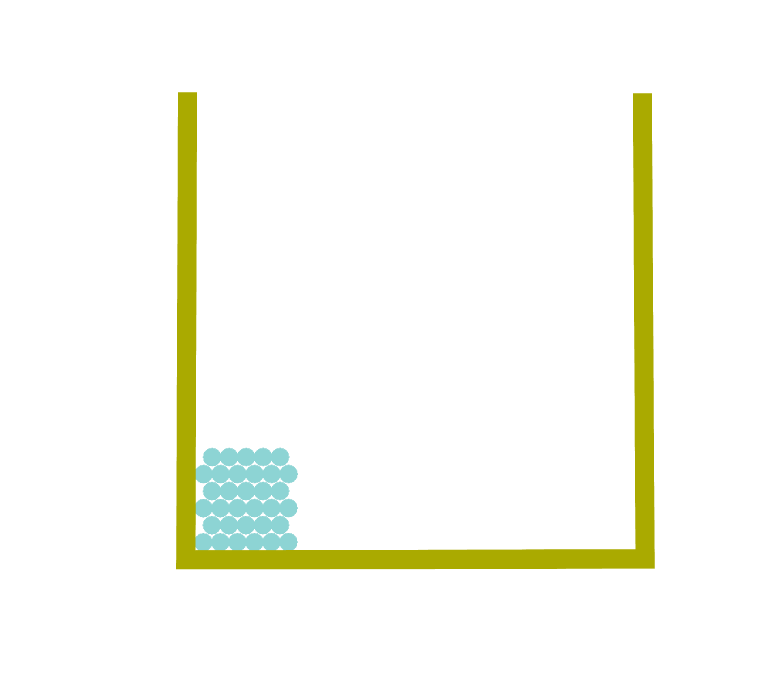
\includegraphics[width=.94\linewidth]{figures/setup.png} 
    \caption{{\small{Case set up in PySPH}}}
    \label{fig:sim_setup}
 \end{subfigure}
 \begin{subfigure}{.5\textwidth}
  \centering
    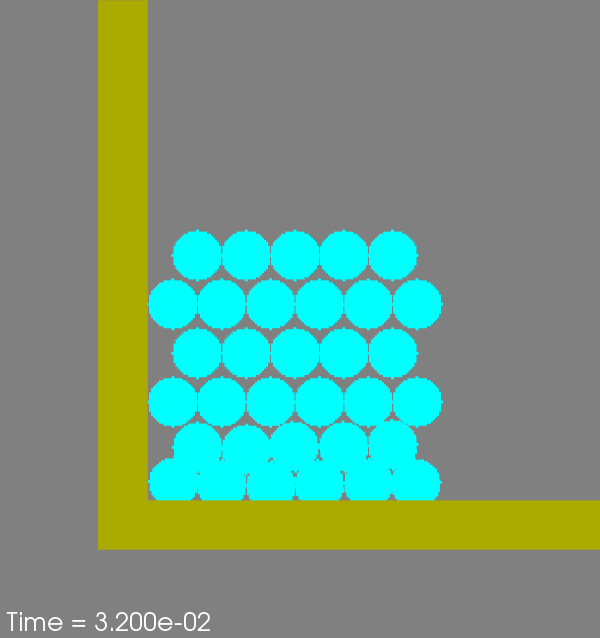
\includegraphics[width=.8\linewidth]{figures/frame000031.png}
    \caption{{\small{System State at time, $t = 0.032 s$}}}
    \label{fig:bestresult_snapshot}
 \end{subfigure}
 \caption{PySPH Validation Study}
\end{figure} % 
 \chapter{The Distributed Contact Discrete Element Method}

The Distributed Contact Discrete Element Method (DCDEM) \cite{canelas} is a variation of the Discrete Element Method wherein the \textbf{Contact Forces }$F^t_i$  acting on the $i^{th}$ particle due to collision with the $j^{th}$ particle is decomposed into \textbf{Normal and Tangential components}  $F_n$ and $F_t$ respectively. Both $F_n$ and $F_t$ are further resolved as \textbf{Repulsive and Dissipative forces},  $F^r$ and $F^d$, coming into existence due to the deformation of the material and the dissipation of energy during the deformation respectively. The DEM mechanisms in two interacting particles is as shown in Figure \ref{fig:dem_mechanism}.

\begin{figure}[htb!]
 \begin{subfigure}{.5\textwidth}
  \centering
    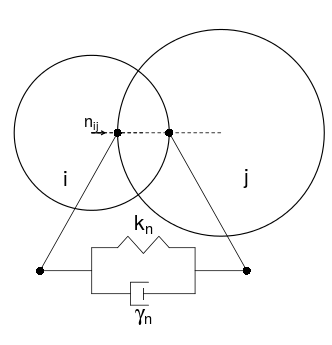
\includegraphics[width=\linewidth]{figures/normal_interaction.png} 
    \caption{{\small{Normal Interation}}}
 \end{subfigure}
 \begin{subfigure}{.5\textwidth}
  \centering
    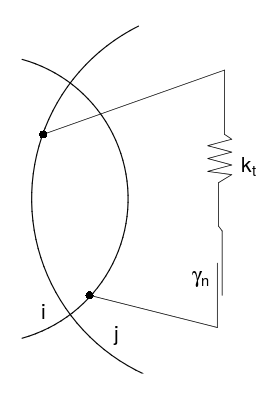
\includegraphics[width=.69\linewidth]{figures/tangential_interaction.png}
    \caption{{\small{Tangential Interaction}}}
     \end{subfigure}
 \caption{Scheme of DEM Mechanism}
 \label{fig:dem_mechanism}
\end{figure}
\newpage
The Normal Contact forces are given by a modified, non-linear Hertzian model as:

\begin{eqnarray}
{\bf{F}} = {\bf{F}}_n^r + {\bf{F}}_n^d = k_{n,ij}~\delta _{ij}^{3/2}~{\bf{e_{ij}}} - \gamma _{n,ij} ~ \delta _{ij}^{1/4} \dot{\delta _{ij}}~\bf{e_{ij}}  
\end{eqnarray}

{\raggedright{where,}}\\
$k_{n,ij} = $ Normal Stiffness Constant of the pair \textit{ij}\\
$\gamma _{n,ij} = $ Normal Damping Constant\\
$\delta _{ij} = $ Particle Overlap $= max(0, \frac{(d_i + d_j)}{2} - {\bf{|{\it{r_{ij}}}|}})$, $d_i, d_j = $ Particle diameter\\
${\bf{e_{ij}}} = $ Unit vector between two mass centers\\
$\dot{\delta _{ij}} = $ Rate of Normal Deformation $= \vec{\it{v_{ij}}}\cdot {\bf{e_{ij}}}$\\

The Stiffness and Damping constants are expressed in terms of the Young's Modulus $E$, Poisson's Ratio $\nu$ and the masses of the $i^{th}$ and $j^{th}$ as:

\begin{eqnarray}
 k_{n,ij} = \frac{4}{3} E^* \sqrt{R^*} \hspace{0.375cm} ; \hspace{0.375cm} \gamma _{n,ij} = C_n \sqrt{6M^*E^* \sqrt{R^*}}
\end{eqnarray}

{\raggedright{where,}}\\
$\frac{1}{E^*} = \frac{1-\nu_I^2}{E_I}+\frac{1-\nu_I^2}{E_I}$ \hspace{0.375cm} ; \hspace{0.375cm} $R^* = \frac{r_i r_j}{r_i + r_j}$ \hspace{0.375cm} ; \hspace{0.375cm} $M^* = \frac{m_I m_J}{m_i + m_j}$\\
with $C_n$ of the order of $10^{-5}$\\


The Tangential Contact Forces are given by Linear Hertzian model bounded by a modified Coulomb Friction Law; the Coulomb Friction Law is modified by means of a sigmoidal function to account for the discontinuity coming into existence when the tangential velocity of the interacting bodies is zero\cite{vetsch}. The model is given as:

\begin{eqnarray}
 {\bf{F}}_{t,ij} = min(\mu_{f,IJ} {\bf{F}}_{n,ij}\tanh(8\dot{\delta^t_{ij}}){\bf{e^t_{ij}}}~; {\bf{F}}_t^r + {\bf{F}}_t^d)
\end{eqnarray}

\hspace{3.15cm}with,

\begin{eqnarray}
 {\bf{F}}_t^r + {\bf{F}}_t^d = k_{t,ij}~\delta^t_{ij}~{\bf{e^t_{ij}}} - \gamma _{t,ij} ~ \dot{\delta ^t_{ij}}~\bf{e^t_{ij}}
\end{eqnarray}

{\raggedright{where,}}\\
$\mu_{f,IJ} = $Coefficient of Kinetic Friction between interacting bodies I and J\\
$\delta^t_{ij} = $ Particle Overlap for Tangential interaction \\
${\bf{e^t_{ij}}} = $ Unit Vector of tangential component of relative velocity perpendicular to $F_n$\cite{vetsch}\\
$k_{t,ij} = $ Tangential Stiffness Constant $= \frac{2}{7} k_{n,ij}$ \cite{hooman}\\
$\gamma_{t,ij} = $ Tangential Damping Constant $=\frac{2}{7} \gamma_{n,ij}$\cite{canelas_thesis}\\
$\dot{\delta ^t_{ij}} = $ Rate of Tangential deformation \\

Since this work makes use of the particle approximation of the SPH method, particle overlap in either the normal or the tangential should be given by the same form; $\dot{\delta ^t_{ij}}$, however, was extrapolated from that of $\dot{\delta _{ij}}$. Thus, the values of the  $\delta^t_{ij}$ and $\dot{\delta ^t_{ij}}$ were taken to be equal to $\delta_{ij}$ and $ \vec{\it{v^t_{ij}}}\cdot {\bf{e_{ij}}}$ respectively. Based on the definition, ${\bf{e^t_{ij}}} = \vec{v_{ij}} - \frac{(\vec{v_{ij}} \cdot \vec{F_{n,ij}}) \vec{F_{n,ij}}}{(|\vec{F_{n,ij}}|^2)}$.

\section{PySPH Implementation}

\subsection{Data Structures and Software Constructs}
As mentioned in Section \ref{sec:pysph_abstractions}, the particle containers can be given additional properties based on the specific requirements of the problem. These are supplied as a ``constants'' dictionary with the keys as the property names and the values as a numpy array. This mechanism is used to provide physical properties such as Young's Modulus, Poisson's Ratio and Coefficient of Kinetic Friction. Further, since the model requires to calculate ${\bf{e_{ij}}}$, the center of masses of all the entities at the initial state of the system are also provided as constants\footnote[9]{The \lstinline!RigidBodyMoments()! class takes care of the evolution of the system mass centers thereafter}. Additionally, in order to demarcate individual solid bodies, the ``body\_id'' constant array is used. 

The interaction between bodies is divided as ``sources'' and ``destinations'', with the ``sources'' contributing to the overall disturbing force on the system and the  ``destinations'' being subjected to those forces. For implementing the new model, the destinations are additionally equipped with five constant arrays: Fx, Fy, Fz, check\_bit, and Fmag. The roles that these arrays play is listed in Table \ref{tab:dest_array}.

\begin{table}[htb!]
\centering
\begin{tabular}{|c|L|}
    \hline
    \textbf{Array Name} & \textbf{Role}\\
             &\\\hline
    Fx       & Array elements hold X Component of Total Collision Force of the destination bodies \\\hline
    Fx       & Array elements hold Y Component of Total Collision Force of the destination bodies \\\hline
    Fx       & Array elements hold Z Component of Total Collision Force of the destination bodies \\\hline
    check\_bit & Binary values of the array elements indicate if the destination body has been considered for force calculation\\\hline
    Fmag     & Magnitude of Maximum Collision Force acting on the destination body \\\hline
\end{tabular}
\caption{\small{Role of Additional Constant Arrays}}
\label{tab:dest_array}
\end{table}

Also, as introduced in section \ref{sec:pysph_abstractions} PySPH has Miscellaneous routines to allow ease in setting up cases and implementing models. These include the \lstinline!loop()! and \lstinline!post_loop()! methods described below:

\begin{itemize}

\item \lstinline!loop()!: This method loops over all the destination array particles ``one by one'' (along with the associated nearest neighbours) in each stage of the integrator step thereby allowing all the necessary force computations on each particle to be performed individually. Each loop cycles through all the 

\item \lstinline!post_loop()!: This method ``loops'' over all the destination array particles ``at once'' in each stage of the integrator step thereby allowing manipulations to all the particles after the individual computations are all completed.
\end{itemize}

The \lstinline!loop()! and \lstinline!post_loop()! methods can take specific arguments as dictated by the physics of the problem. These arguments could be pre-fixed with ``\textbf{s\_}'' and ``\textbf{d\_}'' to associate with the source or destination particle properties. Further, general SPH computations make use of many terms which are common across various domains and are provided as ``Pre-computed Symbols''\footnote[10]{\url{http://pysph.readthedocs.io/en/latest/design/overview.html\#writing-the-equations}} to facilitate easy reuse.

Lastly, as mentioned in Section \ref{sec:pysph_design}, PySPH incorporates Run Time Code Generation (RTCG) to generate C/C++ extensions for all simulations. Therefore, while implementing the model any data structures necessary must be declared such it is parsed and understood by the Cython Code Generator. This can be done by making use of the \lstinline!declare()! function. By default, all explicitly undeclared data structures are treated as pointers to arrays of doubles.

\subsection{Flowchart of DCDEM Implementation}

The flowchart of the implementation is as shown below.  % 
 \chapter{Future Work}

The work presented in this report was largely focussed on getting a physically consistent collision model in place for use within the PySPH framework. This included making a rational choice of the collision model and developing a strategy to implement it in PySPH. However, although literature confirms the verification of the model as laid out by \cite{canelas}, the validity of the PySPH implementation still has to be proven. This is the first task that needs to be addressed in the future.

Further on, once the collision model has been validated, the next task would be to validate a coupled SPH-DCDEM model. Again, the experimental data obtained by \cite{zhang} can be used as a test case. This would then give a complete working scheme to solve Fluid Structure Interaction problems using PySPH. Lastly, another avenue that could be explored is of the coupling of the DCDEM method with the Implicit Incompressible SPH variation of solving SPH equations to give yet another FSI scheme to PySPH users. % 

 \bibliographystyle{apalike} % some standard bibtex style
 \bibliography{report}       % should be in the .bib format
 \addcontentsline{toc}{chapter}{Bibliography}

 % any additional material that belongs to appendices
 \appendix
 \chapter{Case Setup for Validation of RigidBodyCollision Model}\label{app1:case}
\inputminted[fontsize=\scriptsize]{python}{PoC.py}

 
 \chapter{Implementation of DCDEM in PySPH}\label{appendix2}
\inputminted[fontsize=\scriptsize]{python}{DCDEM.py}

 
\end{document}
